\subsection{Modelado del problema}
El modelado del problema es una de los campos con mayor potencial dentro del FJSP, trabajar sobre una 
propuesta solida puede repercutirá directamente en el resultado final, por lo que es necesario
contemplar diferentes alternativas. En este apartado se desarrollará la propuesta final exclusivamente,
pero se hará referencia a otras alternativas que se han descartado dentro de la sección de "Posibles
representaciones del problema".

\subsubsection{Procedimiento para definir un environment de RL}
El RL es un tipo de aprendizaje automático que se basa en la interacción de un agente con el environment. 
Este agente toma decisiones en función de la información que recibe del estado y es recompensado 
o penalizado acorde a las decisiones que toma y su objetivo es maximizar la recompensa total o return
obtenida a lo largo del tiempo. Este tipo de técnicas se pueden utilizar para resolver problemas de optimización 
combinatoria en los que el espacio de estados es muy grande y no es posible explorar todas sus combinaciones. 
En casos en los que el espacio de estado del problema es muy grande o cambia continuamente,
el aprendizaje por refuerzo puede ser útil para encontrar soluciones óptimas sin necesidad de
explorar todo el espacio de estado. Podemos definir un environment de RL formalmente de la siguiente manera:

\begin{itemize}
    \item \textbf{Espacio de estados (S):} Es el conjunto de todos los posibles estados del environment. 
    Puede ser finito o infinito, y se denota como S = \{s1, s2, ..., sn\}, donde si S es finito, n representa 
    el número de estados posibles. Por ejemplo, si estuviéramos modelando un juego de ajedrez, el espacio 
    de estados incluiria todas las posibles configuraciones del tablero.

    \item \textbf{Espacio de acciones (A):} Es el conjunto de todas las posibles acciones que un agente 
    puede tomar en el environment. Al igual que el espacio de estados, el espacio de acciones puede ser finito 
    o infinito, y se denota como A = \{a1, a2, ..., am\}, donde si es finito, m representa el número de 
    acciones posibles. Siguiendo con el ejemplo del juego de ajedrez, el espacio de acciones podría incluir 
    todos los posibles movimientos que un jugador puede hacer en su turno.

    \item \textbf{Función de transición de estados (T):} Es una función que define la probabilidad de transición 
    de un estado a otro estado dado una acción tomada por el agente. Se denota como T(s, a, s'), donde s es el 
    estado actual, a es la acción tomada y s' es el siguiente estado alcanzado después de tomar la acción a en 
    el estado s. Formalmente, la función de transición se puede escribir como: T: S x A x S -> [0, 1], donde 
    [0, 1] representa el rango de probabilidades.

    \item \textbf{Función de recompensa (R):} Es una función que asigna una recompensa numérica a una transición 
    de estado y acción específica. Se denota como R(s, a, s'), donde s es el estado actual, a es la acción tomada, 
    s' es el siguiente estado alcanzado después de tomar la acción a en el estado s, y R(s, a, s') es 
    la recompensa asociada a esa transición. Formalmente, la función de recompensa se puede escribir 
    como: R: S x A x S -> R, donde R es un valor numérico que representa la recompensa. 
\end{itemize}

\textbf{Nota: } En nuestro caso, no será necesario definir una función de recompensa, ya que debido a la 
naturaleza del Imitation Learning no requiere de una función de recompensa. Esto se debe a que el agente 
no toma decisiones por si mismo, sino que aprende a tomar decisiones a partir de un experto.

\subsubsection{Representación del estado}
\paragraph{Representación del estado mediante un grafo heterogéneo}
La propuesta del estado se basa en una representación mediante el uso de un grafo heterogéneo. Un grafo 
heterogéneo es un tipo de grafo en el que los nodos y/o aristas pueden tener diferentes tipos, atributos 
o propiedades. Esto significa que en un grafo heterogéneo se pueden representar diferentes entidades 
o relaciones, y pueden tener diferentes características asociados a ellos. Por ejemplo, en un grafo 
que representa una red social, los nodos pueden representar personas, páginas o grupos y 
las aristas amistades, seguidores, miembros de un grupo, etc.\medskip 

Utilizando un grafo heterogéneo es posible representar tareas, máquinas y trabajos como nodos del grafo, 
mientras que las aristas se utilizan para asignar las restricciones del problema, como los tiempos de 
procesamiento, las dependencias entre tareas y la asignación de tareas. Esto permite una representación 
compacta y eficaz de la información relevante del problema al tratarse de estructuras modulares que 
representan entidades y relaciones en el problema. A medida que se aumenta el número de máquinas y 
operaciones, simplemente se agregarán más nodos y aristas al grafo, lo que no implica un aumento exponencial 
en la complejidad de la representación, permitiendo una escalabilidad natural en términos de la estructura 
del problema. Otra de sus ventajas es que las operaciones sobre grafos, como la búsqueda o manipulación de 
nodos y aristas, son operaciones computacionalmente eficientes. Esto permite realizar cálculos y 
análisis en tiempo razonable, incluso cuando el tamaño del problema se incrementa. 

\begin{table}[ht]
    \caption{Características del nodo Máquina} 
    \centering 
    
    \begin{tabular}{cccccc} 
    \toprule

    \multirow{2}{*}{
    \parbox[c]{.2\linewidth}{\centering Min width}}
      & \multicolumn{2}{c}{$fp_{c}$} &&
    \multicolumn{2}{c}{$fp_{bf}$} \\ 
    \cmidrule{2-3} \cmidrule{5-6}
    
     & {\centering theory} & {exp.} && {theory} & {exp.}  \\
    \midrule
    1 & 0.23  & 0.21  && 0.04               & 0.065 \\
    2 & 0.085 & 0.087 && 0.0015             & 0.0020 \\
    3 & 0.032 & 0.026 && $5.5\times10^{-4}$ & 0 \\
    4 & 0.012 & 0.011 && $5.5\times10^{-4}$ & 0 \\
    \bottomrule

    \end{tabular}
\end{table}


\begin{figure}[ht]
    \centering
    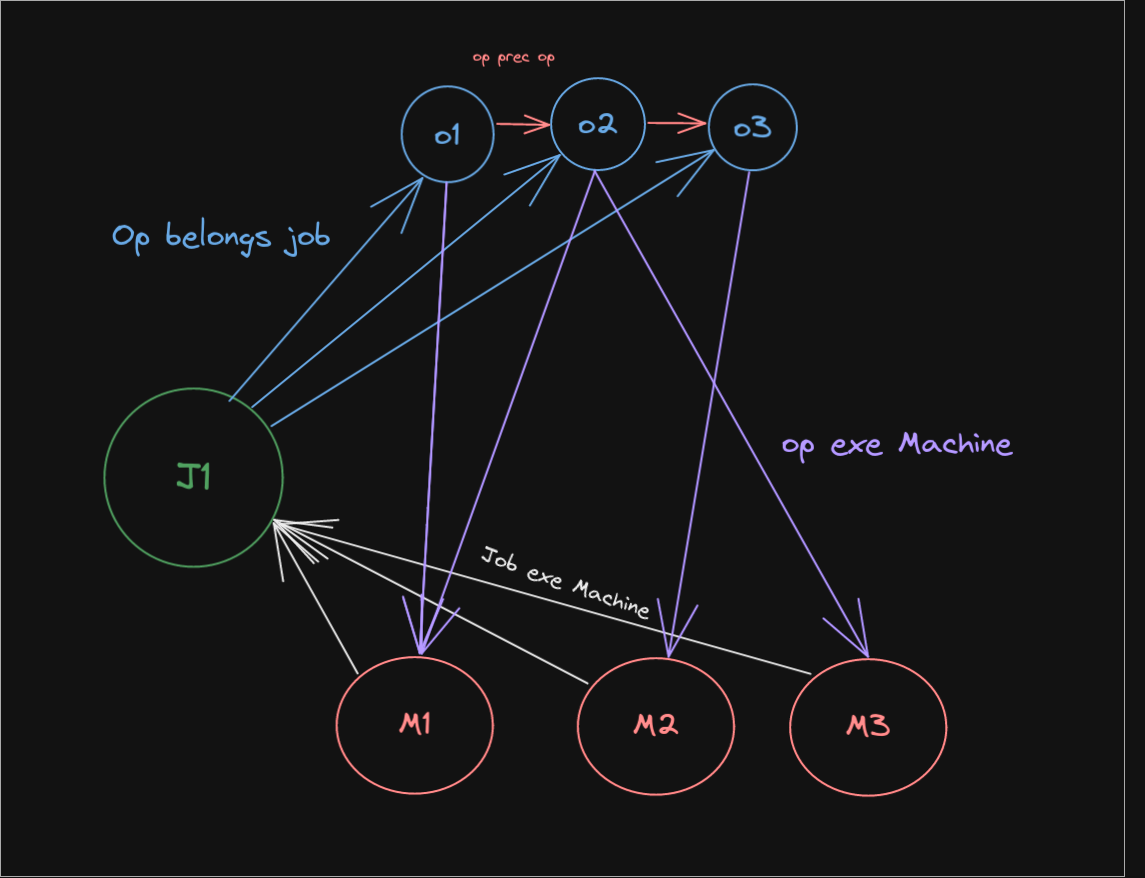
\includegraphics[scale=0.3]{graphv1.png}
    \caption{Diagrama de un environment de RL}
    \label{fig:rl}
\end{figure}

La justificación de usar PyTorch Geometrics es que ofrece soporte para el procesamiento de grafos,
lo que significa que se puede utilizar para trabajar con redes de datos en las que los nodos están
conectados por enlaces. Esto puede ser útil porque mediante técnicas de Deep Learning se puede analizar
la estructura y las relaciones que existen entre los nodos de un grafo. Además, la librería ofrece herramientas
para trabajar con diferentes tipos de grafos, como grafos dirigidos y heterogéneos, que son los utilizados en
nuestra representación, y proporciona una serie de funciones para realizar operaciones básicas con grafos.

\subsubsection{Espacio de acciones}

\subsubsection{Función de transición}

\subsubsection{Función de recompensa}

\pagebreak
